\documentclass[xcolor=dvipsnames]{beamer}
\usetheme{Berlin}  %% Themenwahl
%\definecolor{htwgreen}{rgb}{118,185,0}
\definecolor{htwgreen}{rgb}{0.461,0.723,0}
\definecolor{commentgreen}{rgb}{0,0.6,0}
\definecolor{stringmauve}{rgb}{0.58,0,0.82}
\usecolortheme[named=htwgreen]{structure}

\setbeamertemplate{navigation symbols}{}%remove navigation symbols
%show frame numbers
\expandafter\def\expandafter\insertshorttitle\expandafter{%
\insertshorttitle\hfill%
\insertframenumber\,/\,\inserttotalframenumber}

\usepackage[utf8]{inputenc}
\usepackage[ngerman]{babel} %german language
\usepackage{graphicx} %insert pictures
%\usepackage{svg} %insert vector graphics
\usepackage[export]{adjustbox} %for columns?
\usepackage{listings} %insert code
\lstset{ %configure code listings
	basicstyle=\ttfamily,
	keepspaces=true, 
	numbers=left,
	commentstyle=\color{commentgreen},
	keywordstyle=\color{blue},
	escapeinside={\%*}{*)}
}
\usepackage{tikz} %diagrams
\usepackage{verbatim} %diagrams

\title{Visualisierung der Schwingung einer Gitarrensaite (Wellengleichung)}
\author{Patrick Fehling \& Christian Schütt}
\date{\today}
%**)
\begin{document}
\maketitle
\frame{\tableofcontents}

\section{Grundlagen}
\begin{frame}\frametitle{Aufgabe}
		\textbf{Aufgabe:}\\
		Visualisierung der Amplituden einer vibrierenden Saite auf Grundlage der Wellengleichung im eindimensionalen Fall\\
		\vspace{1ex}
		$A(i, t + 1) = 2A(i, t) - A(i, t - 1) + c(A(i - 1, t) - 2A(i, t) + A(i + 1, t))$\\
		\vspace{2ex}
		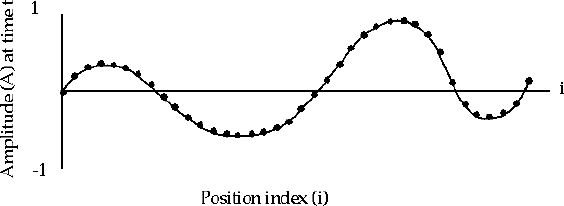
\includegraphics[width=1.0\textwidth,valign=t]{pictures/wellengleichung_aufgabe}
\end{frame}

\begin{frame}\frametitle{Rahmenbedingungen}
	\begin{itemize}
		\item sequentielle Implementierung
		\item parallelisierte Implementierungen
		\item Graphical User Interface
		\item Konfiguration per Benutzeroberfläche oder Konfigurationsdatei
		\item optional: Perturbationen
		\vspace{3ex}
		\item Performancevergleich
		\item Präsentation, Paper, Dokumentation
	\end{itemize}
\end{frame}

\section{Implementierung}
\frame{\tableofcontents[current]}
%Herangehenweise
%Datenstrukturen
%Parallelisierung
%Snippets

\begin{frame}[fragile]\frametitle{Konfiguration}
\begin{lstlisting}[language=Python]
# parameter C in the equation
C 0.1
# shift of sinus function in x orientation
SHIFT 1
# length of the wave
ARRAY_SIZE 1101
# 1 shows GUI; 0 hides GUI
SHOW_GUI 1
# count of simulations (0=infinitely)
SIMULATION_STEPS 0
[...]
\end{lstlisting}
\end{frame}

\begin{frame}[fragile]\frametitle{Berechnung}
\begin{lstlisting}[language=C]
#pragma %*\color{blue}{omp parallel for}*)
for (int i = 1; i < arrLen-1; i++)
{ 
    newval[i] = 2*values[i] - oldval[i] + 
    c*(values[i-1] - 2*values[i] + values[i+1]);
}

#pragma %*\color{blue}{omp parallel for}*)
for (int i = 1; i < arrLen-1; i++)
{ 
    oldval[i] = values[i];
    values[i] = newval[i];
}
\end{lstlisting}
\end{frame}

\begin{frame}\frametitle{Implementierung}
	\centering
	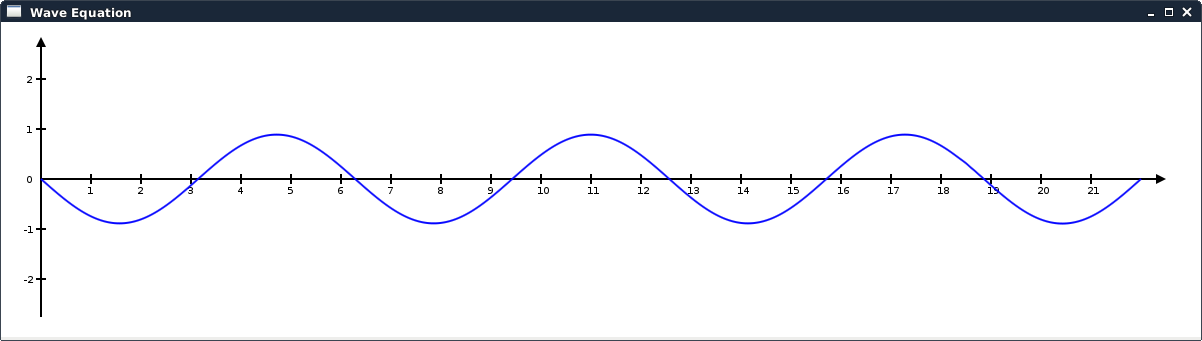
\includegraphics[width=1.0\textwidth,valign=t]{pictures/gui}
\end{frame}

\section{Demo}
\begin{frame}
	\centering
	\textcolor{htwgreen}{{\LARGE Demo}}
\end{frame}

\section{Vergleich}
\frame{\tableofcontents[current]}

\begin{frame}\frametitle{Vergleich}
	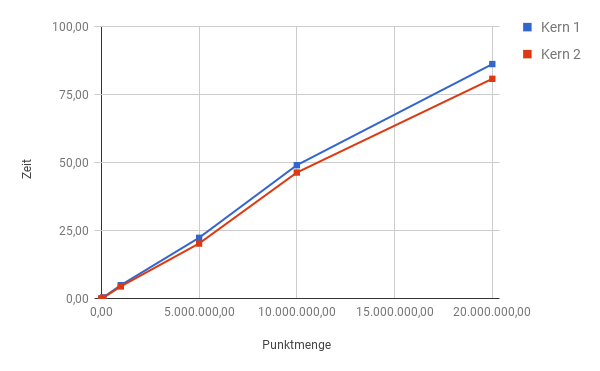
\includegraphics[width=1.0\textwidth,valign=t]{pictures/zeit_punktmenge}
\end{frame}

\begin{frame}\frametitle{Vergleich}
	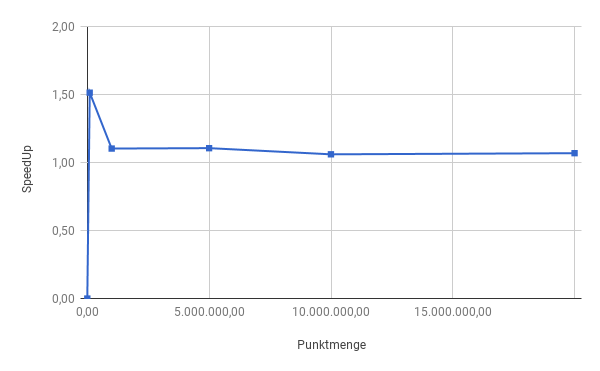
\includegraphics[width=1.0\textwidth,valign=t]{pictures/speedup_punktmenge}
\end{frame}

\section{Fazit \& Ausblick}
\frame{\tableofcontents[current]}

\begin{frame}\frametitle{Fazit}
{\Large 	\begin{itemize}
		\item Parallelisierung mit OpenMP brachte minimale Verbesserung der Laufzeit.\newline
			$\rightarrow$ Zwei parallelisierte Schleifen
	\end{itemize}}
\end{frame}

\begin{frame}\frametitle{Ausblick}
	\begin{itemize}
		\item Falls möglich: Korrektur der OpenMP-Paralellisierung
		\item Implementierung einer zweiten Parallelisierung\newline($\rightarrow$ MPI oder OpenCL)
		\item Implementierung eines Toggles (s. Epidemie)
		\item Analysen mit valgrind und helgrind
		\item optional: Implementierung von Perturbationen, Dämpfung
		\item Erweitern der Konfiguration
		\item Paper \& Dokumentation
	\end{itemize}
\end{frame}

\begin{frame}
	\centering
	\textcolor{htwgreen}{{\LARGE Vielen Dank für Ihre Aufmerksamkeit!\\[6ex] Fragen?}}
\end{frame}

\end{document}